\documentclass[]{scrreprt}
\usepackage{amsmath,amsfonts,graphicx}
\usepackage{multirow}
\usepackage{pslatex}
\usepackage{tabularx}
\usepackage{comment}
\usepackage{xspace}
\usepackage{array}

\usepackage{hyperref}

\usepackage{caption}
\DeclareCaptionFont{white}{\color{white}}
\DeclareCaptionFormat{listing}{\colorbox{gray}{\parbox{\textwidth}{#1#2#3}}}

\graphicspath{
{figures/}
}

\def\species{\mathrm{sp}}
\def\phase{\mathrm{ph}}
\def\massfrac{\chi}
\def\flux{\mathbf{F}}
\def\darcyvel{\mathbf{v}}
\def\energydens{\mathcal{E}}
\def\d{\mathrm{d}}

\newcommand{\uo}{\mbox{UO\textsubscript{2}}\xspace}

\setcounter{secnumdepth}{3}


\begin{document}


\title{Gravity-Head Tests}
\author{CSIRO}
\maketitle

\tableofcontents

\chapter{Establishment of gravity head in 1D}

These tests concern the steadystate pressure distribution obtained
either by running a transient model for a long time, or by running a
steady-state analysis, both of which should lead to the same result.
Without fluxes, the steadystate pressure distribution is just
\begin{equation}
P(x) = P_{0} - \rho_{0} g x \ ,
\end{equation}
if the fluid bulk modulus, $B$, is large enough compared with $P$.
Here $P_{0}$ is the porepressure at $x=0$.  For smaller bulk modulus
\begin{equation}
P(x) = -B \log\left( e^{-P_{0}/B} + \frac{g\rho_{0}x}{B} \right) \ .
\label{grav.head.eqn}
\end{equation}
Here it is assumed that the density is given by $\rho = \rho_{0}e^{-P/B}$
with constant bulk modulus, $g$ is the
magnitude acceleration due to gravity (a vector assumed to be pointing in the
negative $x$ direction), and $x$ is position.  The tests described below
are simple tests and are part of the automatic test suite.

\section{Single-phase, single-component}
\label{1phase1comp.sec}

Two single-phase simulations with 100 1D elements are run: one with
fully-saturated conditions, and the other with unsaturated conditions
using the van-Genuchten capillary pressure (this should not, and does
not, make any difference to the results).  The porepressure is held
fixed at one boundary ($x=0$).

An example verification is shown in Figure~\ref{gh.fig}, which also
shows results from a 2-phase simulation (see Section~\ref{2phase.sec}).

\begin{figure}[htb]
\centering
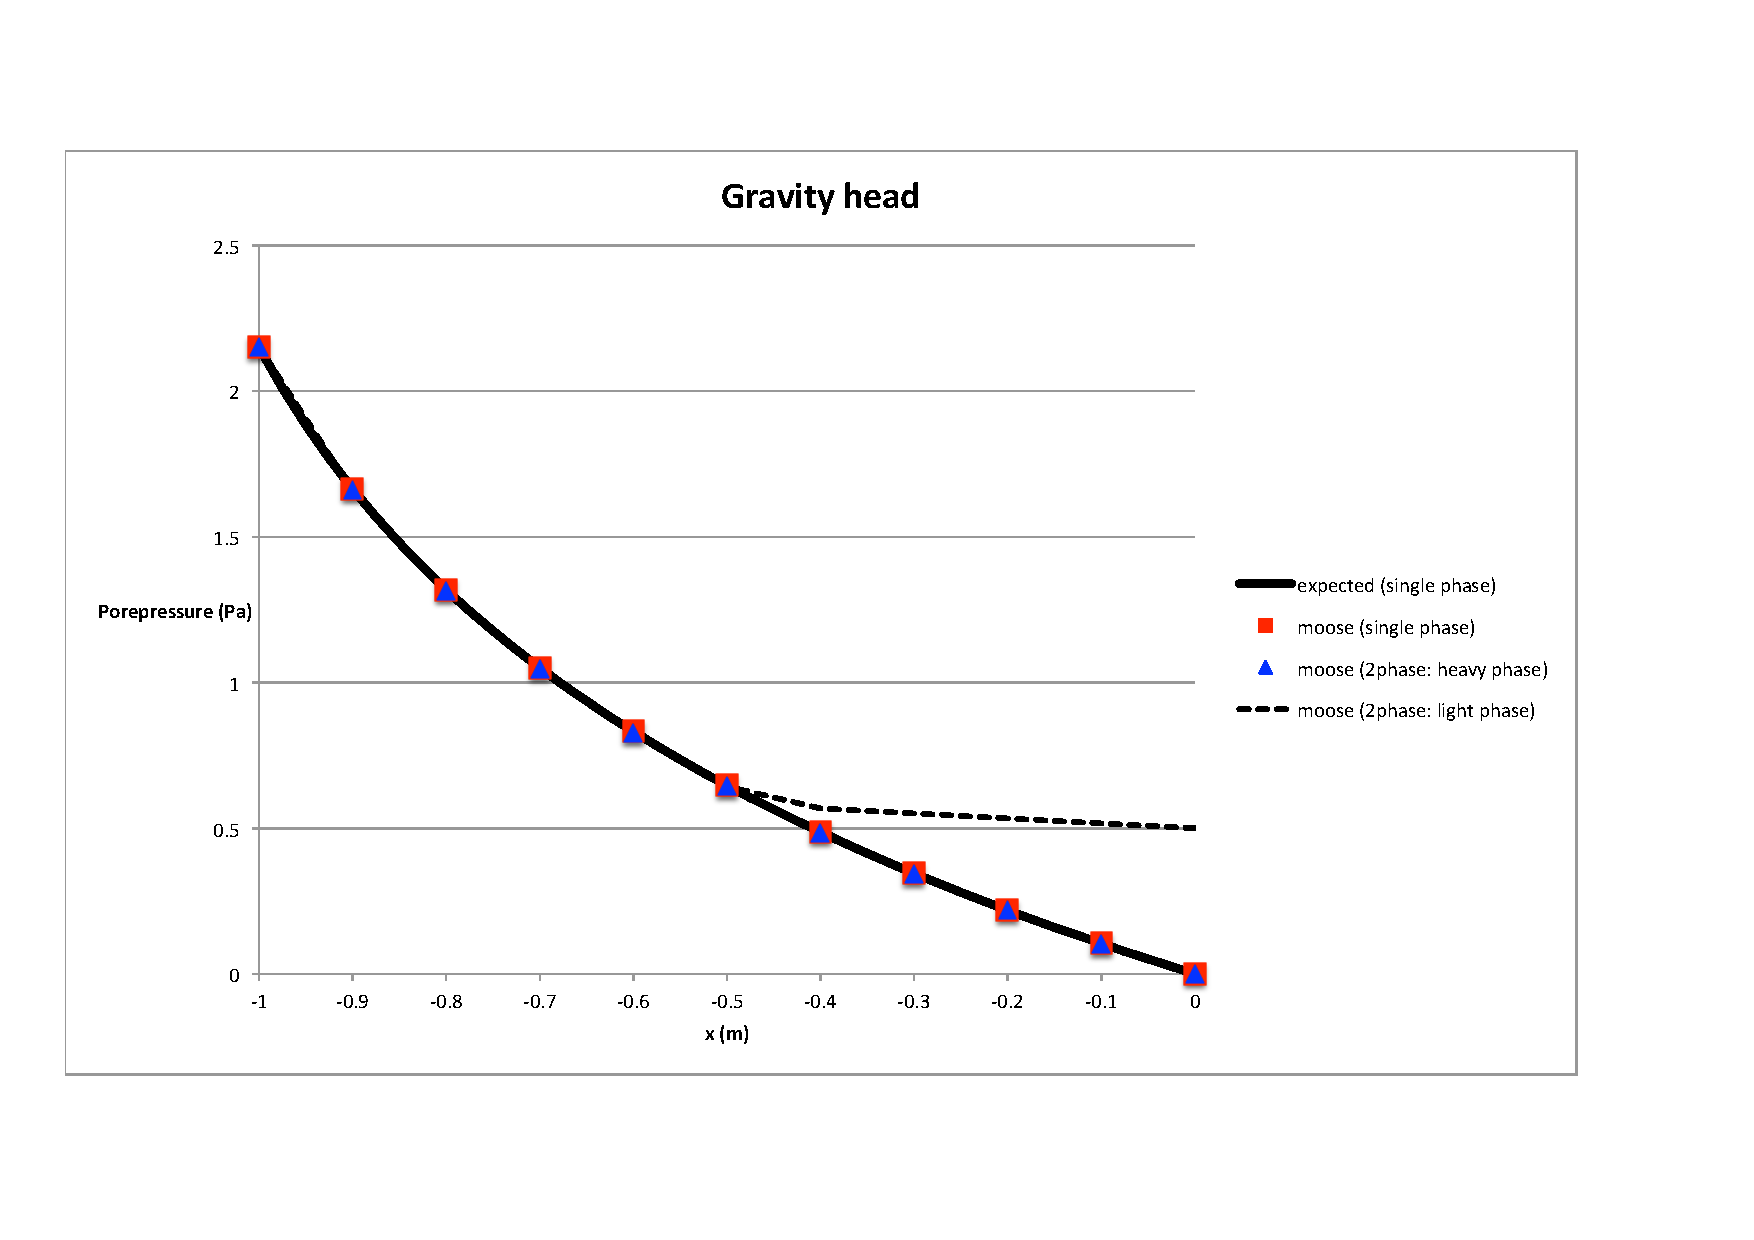
\includegraphics[width=15cm]{gravity_fig.pdf}
\caption{Comparison between the MOOSE result (in dots), and the
  exact analytic expression given by Eqn~(\ref{grav.head.eqn}).
  test had 10 elements in the $x$ direction, with $-1\leq x \leq
  0$\,m.  The parameters were $B=1.2$\,Pa, $\rho_{0}=1$\,kg.m$^{-3}$,
  and $g=-1$\,m.s$^{-2}$.  For the two-phase simulation, the light
  phase had $B=1$\,Pa and $\rho_{0}=0.1$\,kg.m$^{-2}$.}
\label{gh.fig}
\end{figure}

\section{Two-phase, two-component}
\label{2phase.sec}

Two-phase, two-component simulations may also be checked against
Eqn~(\ref{grav.head.eqn}).  Four simulations are performed.

One steady-state simulation is performed.  Steady-state simulations are more
difficult to perform in two-phase situations because of the inherently
stronger nonlinearities, but mostly because simulations can easily enter
unphysical domains (negative saturation, for instance) without the stabilising
presence of the mass time-derivative.

Three transient simulations are performed.  In the
transient simulations, conservation of mass can be checked, and the
tests demonstrate MOOSE conserves mass.  Depending on the initial and
boundary conditions, the ``heavy'' phase (with greatest mass) can
completely displace the ``light'' phase, which is forced to move to
the top of the simulation.  In this case Eqn~(\ref{grav.head.eqn})
only governs the light phase in the unsaturated zone, since in the
saturated zone (where there is zero light phase) the pressure must
follow the heavy-phase version of Eqn~(\ref{grav.head.eqn}).  An
example is shown in Figure~\ref{gh.fig}.



\end{document}

